%%%%%%%%%%%%%%%%%%%%%%%%%%%%%%%%%%%%%%%%%%%%%%%%%%%%%%%%%%%%%%%%%%%%%%%%%%%%%%%%%%%%%%%%%%%%%%
%
% MASTER THESIS
%
% This is the main .tex-document for my master thesis.
% In here only belong necessary things, such as the declaration of the document class.
% Everything else is supposed to be in seperate files which are then included via \input.
% Have fun writing!
%
% Fabian Burghart, 2018/02/17
%
%%%%%%%%%%%%%%%%%%%%%%%%%%%%%%%%%%%%%%%%%%%%%%%%%%%%%%%%%%%%%%%%%%%%%%%%%%%%%%%%%%%%%%%%%%%%%%

\RequirePackage[l2tabu, orthodox]{nag}
\documentclass[a4paper,11pt,twoside,notitlepage]{report}
\usepackage[a4paper, inner=3cm, outer=2cm, top=3cm, bottom=3cm]{geometry}

\usepackage[utf8]{inputenc}
\usepackage[T1]{fontenc}
\usepackage{lmodern}

% Remaining packages %
%%%%%%%%%%%%%%%%%%%%%%%%%%%%%%%%%%%%%%%%%%%%%%%%%%%%%%%%%%%%%%%%%%%%%%%%%%%%%%%%%%%%%%%%%%%%%%
%
% MASTER THESIS
%
% This is the first part of the preamble for my master thesis.
% In here only belong packages which are not already included in mt_main.tex, 
% and options tied to them.
% Have fun writing!
%
% Fabian Burghart, 2018/02/17
%
%%%%%%%%%%%%%%%%%%%%%%%%%%%%%%%%%%%%%%%%%%%%%%%%%%%%%%%%%%%%%%%%%%%%%%%%%%%%%%%%%%%%%%%%%%%%%%

\usepackage[english]{babel}			%language

\usepackage[style=alphabetic,backend=biber]{biblatex}
\usepackage{csquotes}
\usepackage{graphicx}				%pictures
\usepackage{tikz}				%drawing
\usepackage{paralist}				%options on enumerating
\usepackage{fancyhdr}				%header/footer
\usepackage[hidelinks,pdfpagelabels]{hyperref}		%allowing links (hidden, for esthetic reasons)
\usepackage{color}				%allows using colors

% Mathematics %

\usepackage{amsmath}				%maths
\usepackage{amssymb}				%symbols 
\usepackage{amsthm}				%theorems

\usepackage{mathtools}				%more maths
\usepackage{mathrsfs}				%fancy letters
\usepackage{dsfont}				%variations of double-stroked letters

% Esthetic %

\usepackage{booktabs}				%nicer tables
\usepackage{setspace}				%space between lines
\usepackage{microtype}				%optimizing text

\pagestyle{fancy}				%page layout
\setlength{\headheight}{16pt}
\lhead{}
\chead{\leftmark}
\rhead{}
\lfoot{}
\cfoot{\thepage}
\rfoot{}


% Options and shortcuts %
%%%%%%%%%%%%%%%%%%%%%%%%%%%%%%%%%%%%%%%%%%%%%%%%%%%%%%%%%%%%%%%%%%%%%%%%%%%%%%%%%%%%%%%%%%%%%%
%
% MASTER THESIS
%
% This is the first part of the preamble for my master thesis.
% In here only belong options such as shortcuts, macros, new environments, etc.
% Have fun writing!
%
% Fabian Burghart, 2018/02/17
%
%%%%%%%%%%%%%%%%%%%%%%%%%%%%%%%%%%%%%%%%%%%%%%%%%%%%%%%%%%%%%%%%%%%%%%%%%%%%%%%%%%%%%%%%%%%%%%

%% GENERAL OPTIONS %%

\setlength\parindent{0pt}   %Better paragraphs
\setlength{\parskip}{4pt}

\setstretch{1.1}



%% NEWCOMMANDS %%

% doublestroke

\newcommand{\IR}{\mathbb{R}}

% greek

\newcommand{\ga}{\alpha}
\newcommand{\gd}{\delta}
\newcommand{\gD}{\Delta}
\newcommand{\gl}{\lambda}
\newcommand{\gs}{\sigma}
\newcommand{\go}{\omega}
\newcommand{\gO}{\Omega}

% mathcal

\newcommand{\cA}{\mathcal{A}}
\newcommand{\cB}{\mathcal{B}}
\newcommand{\cH}{\mathcal{H}}

% mathscr

\newcommand{\scA}{\mathscr{A}}
\newcommand{\scB}{\mathscr{B}}
\newcommand{\scF}{\mathscr{F}}

% dimensions & related

\newcommand{\diam}{\operatorname{diam}}
\newcommand{\dimh}{\dim_{\mathcal{H}}}  %Hausdorff dimension
\newcommand{\dims}{\dim_{\mathcal{S}}}  %spectral dimension
\newcommand{\dimw}{\dim_{\mathcal{W}}}  %walk dimension

% math symbols

\newcommand{\ssq}{\subseteq}
\newcommand{\Di}{\operatorname{d}\!}
\newcommand{\Prob}{\mathbf{P}}




%% ENVIRNOMENTS %%

\makeatletter
\newtheoremstyle{defindented}
  {3pt}% space before
  {3pt}% space after
  {\addtolength{\@totalleftmargin}{1em}
   \addtolength{\linewidth}{-2em}
   \parshape 1 1em \linewidth}% body font
  {}% indent
  {\bfseries}% header font
  {.}% punctuation
  {.5em}% after theorem header
  {}% header specification (empty for default)
\makeatother

\makeatletter
\newtheoremstyle{thmindented}
  {3pt}% space before
  {3pt}% space after
  {\addtolength{\@totalleftmargin}{1em} \itshape
   \addtolength{\linewidth}{-2em}
   \parshape 1 1em \linewidth}% body font
  {}% indent
  {\bfseries}% header font
  {.}% punctuation
  {.5em}% after theorem header
  {}% header specification (empty for default)
\makeatother

\theoremstyle{thmindented}
\newtheorem{prop}{Proposition}[chapter]
\theoremstyle{defindented}
\newtheorem{defin}[prop]{Definition}




% Bibliography
\addbibresource{mt_bib.bib}

% Title Page

\title{$\ $\\ \textsc{The Einstein Relation on Fractals and Other Singular Sets}\\$\ $}
\author{{\Large {Fabian Burghart}}\\[1em]
  {\large April 2, 2018}\\[10em]}
\date{{\large Master thesis in mathematics}\\
  {\large Advisor: Prof. Dr. Uta Renata Freiberg}\\[7em]
  {\large \textsc{Fakult{\"a}t f{\"u}r Mathematik und Physik der Universit{\"a}t Stuttgart}}} 

%%%%%%%%%%%%%%
%% DOCUMENT %%
%%%%%%%%%%%%%%

\begin{document}
\maketitle
\thispagestyle{empty}
\newpage

\thispagestyle{empty}

\section*{Preface: Beware of construction works!}

This is an early draft of my Master thesis on the so-called Einstein relation. ``Early'' because I started working on the topic after the German winter term finished (which was mid-February at my university) and since spent most of my time reading literature to understand the existing theory. Accordingly, a lot of the ideas I currently have are not yet worked out completely, a lot of the text is still unrefined, pictures for the examples in chapter 2 are non-existent, there are several gaps in the material that still have to be filled out - and even the title might be subject to future changes. However, I added short remarks denoted by ``TO DO'' to signify my overall plans, and I do hope that this current draft - despite admittedly resembling a desolate construction site more than a newly finished building - fulfills the needs as part of this application.

\begin{flushright}
  Fabian Burghart, 22nd April 2018. 
\end{flushright}


\tableofcontents


% Chapter I. An introduction to the Einstein Relation
\chapter{Fractal Dimensions and the Einstein Relation}

In this introductory chapter, we wish to briefly expose the ingredients of the Einstein relation - the Hausdorff dimension $\dimh$, the spectral dimension $\dims$, and the walk dimension $\dimw$ - and state some of their properties. 

\section{Hausdorff measure and Hausdorff dimension}

Although the concepts of Hausdorff measure and dimension are well-known, we give the definitions in the interest of completeness. In what follows, let $(X,d)$ be a metric space.
\begin{defin}[Hausdorff outer measure]
  For fixed $s\geq0$, any subset $S\ssq X$ and any $\gd>0$, let 
  \[
    \cH^s_\gd(S)
      :=\inf \left\{\sum_{i\in I}(\diam U_i)^s:
            |I|\leq\aleph_0,S\ssq\bigcup_{i\in I}U_i\ssq E,\diam U_i\leq\gd\right\},
  \]
  i.e. the infimum is taken over all countable coverings of $S$ with diameter at most $\gd$. The $s$-dimensional Hausdorff outer measure of $S$ is now defined to be
  \begin{equation}\label{eq:DHM}
    \cH^s(S):=\lim_{\gd\searrow0}\cH^s_\gd(S).
  \end{equation}
\end{defin}
Observe that the limit in \eqref{eq:DHM} exists or equals $\infty$, since $\cH^s_\gd(S)$ is monotonically nonincreasing in $\gd$ and bounded from below by 0. Furthermore, it can be shown that $\cH^s$ defines a metric outer measure on $X$, and thus restricts to a measure on a $\gs$-algebra containing the Borel $\gs$-algera $\scB(X)$ (cf. \cite[p.54ff]{mattila1999geometry}). By definition, the obtained measure then is the $s$-dimensional Hausdorff measure which we will denote by $\cH^s$ as well. Note that for $\cH^s$ to be a Radon measure, i.e. locally finite and inner regular, $\cH^s(X)<\infty$ is sufficient.

In the special case of $(X,d)$ being an Euclidean space, Hausdorff measures interpolate between the usual Lebesgue measures $\gl^n$: For $s=0$, we have simply $\cH^0(S)=\# S$, whereas for any integer $n>0$, it can be shown that there exists a constant $c_n>0$ depending only on $n$ such that $\cH^n=c_n\gl^n$, where the constant is the volume of the $n$-dimensional unit ball.

It can be seen by simple estimates that the map $s\mapsto \cH^s(S)$ for fixed $S\ssq X$ is monotonically nonincreasing. More specifically, if $\cH^s(S)$ is finite for some $s$ then it vanishes for all $s'>s$, and conversely, if $\cH^s(S)<\infty$ then $\cH^{s'}(S)=\infty$ for all $s'<s$. Therefore, there exists precisely one real number $s$ where $\cH^\cdot(S)$ jumps from $\infty$ to $0$ (by possibly attaining any value of $[0,\infty]$ there). This motivates the following definition of Hausdorff dimension:
\begin{defin}
  The Hausdorff dimension $\dimh(S)$ of $S\ssq X$ is defined as
  \[
    \dimh(S):=\inf\{s\geq0:\cH^s(S)<\infty\}.
  \]
\end{defin}
Due to the above discussion, we have the following equalities:
\begin{align*}
   \dimh(S)&=\inf\{s\geq0:\cH^s(S)<\infty\}=\inf\{s\geq0:\cH^s(S)=0\}\\
           &=\sup\{s\geq0:\cH^s(S)=\infty\}=\sup\{s\geq0:\cH^s(S)>0\},
\end{align*}
providing some alternative characterisations of the Hausdorff dimension.

We further collect some important facts. To this end, let $S,S'$ and $S_1,S_2,...$ be subsets of $E$ as before. Then, the following properties hold (cf. \cite[p.32f]{falconer2007fractal} for a discussion in the Euclidean setting; however all arguments adapt to our more general situation without complication):
\begin{compactdesc}
  \item[Monotonicity.] If $S\ssq S'$ then $\dimh(S)\leq\dimh(S')$. 
  \item[Countable Stability.] For a sequence $(S_n)_{n\geq1}$, we have the equality
  \[ 
    \dimh\left(\bigcup_{n\geq1}S_n\right)=\sup_{n\geq1} \dimh(S_n).
  \]
  \item[Countable Sets.] If $|S|\leq\aleph_0$ then $\dimh(S)=0$.
  \item[H\"older continuous maps.] If $(X',d')$ is another metric space and $f:X\to X'$ is $\ga$-H\"older continuous for some $\ga\in(0,1]$ then $\dimh(f(S))\leq \ga^{-1}\dimh(S)$. In particular, the Hausdorff dimension is invariant under a bi-Lipschitz transformation (i.e. an invertible map $f$ with H\"older exponent $\ga=1$ for both $f$ and $f^{-1}$).
  \item[Euclidean Case.] If $(X,d)$ happens to be an Euclidean space (or more generally a continuously differentiable manifold) of dimension $n$ and $S$ is an open subset then $\dimh(S)=n$.
\end{compactdesc}

We conclude this section by citing Hutchinson's theorem about the Hausdorff dimension of self-similar sets which will provide us with a plethora of interesting examples. For this, we recall that a map $F:X\to X$ on a metric space $(X,d)$ is a strict contraction if its Lipschitz constant satisfies
\begin{equation}\label{eq:Lip}
  \Lip_F:=\sup_{\stackrel{x,y\in X}{x\neq y}}\frac{d(F(x),F(y))}{d(x,y)}<1.
\end{equation}
If the stronger condition $d(F(x),F(y))=\Lip_F d(x,y)$ holds for all $x,y\in X$, we call $F$ a similitude with contraction factor $\Lip_F$.
\begin{thm}[Hutchinson, \cite{hutchinson1981fractals}]\label{thm:hutchinson}
  Let $\scS=\{S_1,...,S_N\}$ be a finite set of strict contractions on the Euclidean space $\IR^n$. Then there exists a unique nonempty compact set denoted by $|\scS|$ which is invariant under $\scS$, i.e.
  \[
    |\scS|=\bigcup_{i=1}^N S_i(|\scS|).
  \]
  Furthermore, assume that $|\scS|$ satisfies the open set condition (OSC) meaning that there exists a nonempty open set $O\ssq E$ with the properties $S_i(O)\ssq O$ and $S_i(O)\cap S_j(O)=\emptyset$ for all $i,j=1,...,N$ with $i\neq j$. Also assume that the maps $S_i$ are similitudes with contraction factor $r_i\in(0,1)$. Then, $s=\dimh(|\scS|)$ is the unique solution to the equation
  \[
    \sum_{i=1}^N r_i^s=1
  \]
  and we have $0<\cH^s(|\scS|)<\infty$. 
\end{thm}
While uniqueness and existence of $|\scS|$ are still ensured for maps on a complete metric space, the open set condition is not sufficient for statements about the Hausdorff dimension, see \cite{schief1996self} for further discussion. 



\section{Weyl asymptotics and spectral dimension}

The idea of introducing spectral dimension is inspired by Weyl's law for the eigenvalues of the Dirichlet-Laplace operator which we will discuss here shortly.

\subsection{The classical case}

Given a bounded open domain $E\ssq\IR^n$, consider the Laplace operator $\gD$ on $E$ acting on functions satisfying the Dirichlet boundary condition $u\equiv0$ on $\partial E$. Then, the spectrum of $-\gD$ consists of non-negative eigenvalues with a single limit point at $\infty$. Hence we can order them in a non-increasing way, counting the geometric multiplicities, as
\begin{equation}\label{eq:EVs}
  0\leq\gl_1\leq\gl_2\leq...\leq\gl_n\leq...\ \text{ with }\ \gl_n\nearrow\infty. 
\end{equation}
In this setting, it makes sense to define the eigenvalue counting function via 
\begin{equation}\label{eq:DECF}
  N_{-\gD}(x):=\max\{n\in\IN:\gl_n\leq x\},\ x\in\IR_{\geq0}.
\end{equation}
Weyl's law now states that there is the asymptotic equivalence\footnote{We adopt the notation $f\sim g$ for the equivalence relation given by $\lim\frac{f}{g}=1$.}
\begin{equation}\label{eq:WL}
  N_{-\gD}(x)\sim C_n\cH^n(E)x^{n/2},\quad x\nearrow\infty,
\end{equation}
where the constant $C_n$ is independent of the domain $E$ (see \cite{Weyl1911} and \cite{Weyl1912} for the original publications). Motivated by \eqref{eq:WL}, we define the spectral dimension of $-\gD$ on $E$ by
\begin{equation}\label{eq:dims}
  \dims(E,-\gD):=\lim_{x\to\infty}\frac{\log N_{-\gD}(x)}{\log x}
\end{equation}
which yields $n/2$ in the situation examined by Weyl's law. Note that the usual definition of $\dims$ differs by a factor of 2 (cf. \cite{kigami1993weyl},\cite{hambly_kigami_kumagai_2002}) so that $\dims(E,\gD)$ normally coincides with $\dimh(E)=n$, however coming at the cost of an additional factor in the Einstein relation. Moreover, it can be argued that the spectral dimension is rather a property of the operator $-\gD$ than of the underlying space $E$. Therefore, we take the liberty to deviate from the established convention in this minor aspect.

\subsection{The general case}

How can we generalise the concepts just introduced to sets $E$ which are not bounded open subsets of $\IR^n$? For this, suppose we are given a metric measure space $(E,d,\mu)$, where $(E,d)$ is a locally compact separable metric space and $\mu$ is a Radon measure on $E$.

Of course, the notion of an eigenvalue counting function as outlined above works for any operator $A$ whose set of eigenvalues possesses only one limit point at $+\infty$. However, as we will explain in the next section, we also wish to associate a reasonably well-behaved Markov process with state space $E$ to $A$. Therefore, we choose to impose the following conditions on $A$:
\begin{cond}\label{cond:A}
For an operator $A:L^2(E,d)\supseteq\cD(A)\to L^2(E,d)$, we assume the following holds:
\begin{compactdesc}
  \item[Self-adjointness.] $A$ is a densely defined, self-adjoint operator on the Hilbert space $L^2(E,\mu)$.
  \item[Eigenvalues.] The spectrum is contained in $\IR_{\geq0}$ and the set of eigenvalues can be enumerated as in \eqref{eq:EVs}.
  \item[Dissipativeness.] $-A$ is dissipative. In other words, for all $f\in\cD(A)$ and all $\gl>0$, we have 
  $\|(\gl+A)f\|\geq\gl\|f\|$.
\end{compactdesc}
\end{cond}
The first of these assumptions guarantees that $A$ is a closed operator, whereas the second ensures that $\gl+A$ is surjective for at least one $\gl>0$. Thus, the Hille-Yosida theorem states that there is a strongly continuous semigroup of contractive linear operators $T_t$ on $H$ such that $-A$ is its infinitesimal generator. That is to say:
\begin{defin}\label{def:semigroup}
  A strongly continuous semigroup $(T_t)_{t\geq0}$ on a Hilbert space $H$ is a monoid homomorphism $t\mapsto T_t$ from $(\IR_{\geq0},+)$ to the space of bounded linear operators $(\IB(H),\cdot)$ on $H$ (equipped with composition) satisfying for all $f\in H$ the additional property
  \[
    \lim_{t\searrow0} \|T_tf-f\|=0.
  \]
  The infinitesimal generator $(-A,\cD(A))$ of $(T_t)_{t\geq0}$ is defined via
  \[
    (-A)f=\lim_{t\searrow0}\frac{1}{t}(T_tf-f),\ f\in\cD(A),
  \]
  where $\cD(A)$ is the set of elements in $H$ for which this limit exists.
\end{defin}
\begin{thm}[Hille--Yosida]\label{thm:HY}
  An operator $(-A,\cD(A))$ is the generator of a strongly continuous semigroup $(T_t)_{t\geq0}$ with $\|T_t\|\leq1$ for all $t\geq0$ if and only if $-A$ is a densely defined, closed, dissipative operator such that for some $\gl>0$, the map $\gl+A$ is surjective. 
\end{thm}
It can be shown that there is a one-to-one correspondence between contractive semigroups and operators that satisfy the Hille-Yosida theorem, that is, the semigroup in the above theorem is uniquely determined by $A$. 

Having discussed the motivation for the assumptions \ref{cond:A}, we now proceed to adapt the definitions made in \eqref{eq:DECF} and \eqref{eq:dims} in a rather straightforward way:
\begin{defin}
  Given an operator $(A,\cD(A))$ on $L^2(E,\mu)$ satisfying the assumptions \ref{cond:A}, its eigenvalue counting function is defined by
  \begin{equation}\label{eq:defEVCF}
    N_A(x):=\max\{n\in\IN:\gl_n\leq x\},\ x\in\IR_{\geq0},
  \end{equation}
  and the spectral dimension of $A$ by
  \begin{equation}\label{eq:defdims}
    \dims(E,A):=\lim_{x\to\infty}\frac{\log N_A(x)}{\log x}.
  \end{equation}
\end{defin}

TO DO: Provide examples for operators satisfying assumptions 1.4 - e.g. one-sided inverses of injective bounded compact operators. Also, streamline those assumptions, as of now, they are somewhat redundant. Stronger emphasis on Feller semigroups might also be needed, since Dynkin's probabilistic characterisation of the generator \cite[Theorem 19.23]{kallenberg2002foundations} might help in providing some general results concerning the validity of the Einstein relation.


\section{Markov processes and walk dimension}

\subsection{From Dirichlet forms to Markov processes}

The theory presented here is mostly taken from \cite{fukushima2011dirichlet} and \cite[ch. 4]{ma2012introduction}. Set $H=L^2(E,\mu)$ where $\mu$ is a $\gs$-finite Borel-measure on $E$. 
\begin{defin}\label{defin:DF}
  A map $\cE:\cD(\cE)\times\cD(\cE)\to\IR$ is a Dirichlet form if it satisfies the following conditions:
  \begin{compactenum}[i.]
  \item The domain $\cD(\cE)\ssq H$ of $\cE$ is a dense linear subspace.
  \item $\cE$ is a symmetric, non-negative definite bilinear form.
  \item This form is closed, that is, the inner product space $(\cD(\cE),\cE_\ga)$ equipped with the scalar product
  \[
    \cE_\ga(u,v):=\cE(u,v)+\ga\left<u,v\right>\ \text{ for }\ u,v\in\cD(\cE_\ga)=\cD(\cE),\ \ga>0,
  \]
  is complete (and thus itself a Hilbert space).
  \item $\cE$ is a Markovian form, i.e. for all $u\in\cD(\cE)$, $v:=(0\vee u)\wedge 1\in\cD(\cE)$ and we have $\cE[v]\leq\cE[u]$ for the quadratic form of $\cE$. 
  \end{compactenum}
\end{defin}
We remark that the choice of $\ga>0$ is irrelevant for the completeness of $(\cD(\cE),\cE_\ga)$ since all induced norms are equivalent to each other. 
\begin{defin}
  A Dirichlet form $(\cE,\cD(\cE))$ on $L^2(E,\mu)$ is said to be
  \begin{compactenum}[i.]
    \item regular if it possesses a core, that is, the space $\cD(\cE)\cap C_c(E)$ is simultaneously dense in $\cD(\cE)$ with respect to the $\cE_1$-norm and in $C_c(E)$ with respect to the uniform norm. 
    \item local if $\cE(u,v)=0$ whenever $u,v\in\cD(\cE)$ have disjoint compact support.
    \item strongly local if $\cE(u,v)=0$ whenever $u,v\in\cD(\cE)$ have compact support and $v$ is constant on a neighbourhood of $\supp(u)$.
  \end{compactenum}
  If additionally $\mu(E)<\infty$, we say that $\cE$ is
  \begin{compactenum}[i.]
    \setcounter{enumi}{3}
    \item conservative if $1\in\cD(\cE)$ and $\cE[1]=0$.
    \item irreducible if it is conservative and $\cE[f]$ implies that $f$ is constant. 
  \end{compactenum}
\end{defin}
We can uniquely attach a positively semidefinite operator $A$ to a Dirchlet form (and vice versa) via the relation 
\begin{equation}\label{eq:DFtoOp}
  \cE(u,v)=\left<Au,v\right>,\  u\in\cD(A),v\in\cD(\cE).
\end{equation}
In particular, if $A$ meets the requirements of \ref{cond:A}, we not only have precisely one strongly continuous contraction semigroup on $H$ as explained by theorem \ref{thm:HY}, but also a unique Dirichlet form thanks to \eqref{eq:DFtoOp}. In similar style, we would also like to attach a unique Markov process to $A$ - or, equivalently, to the semigroup or the Dirichlet form. 

To define a suitable stochastic process with values in $E$, we first adjoin a cemetary state $*$ in such a way that if $E$ is non-compact, $E_*:=E\sqcup\{*\}$ is the one-point compactification of $E$, whereas $*$ is supposed to be an isolated point if $E$ is compact. Let $X=\left(\gO,\scA,(X_t)_{t\geq0},(\Prob_x)_{x\in E_*}\right)$ be a stochastic process on a measurable space $(\gO,\scA)$ with values in $E_*$, where we adapt the notation that $\Prob_x[X_0=x]=1$ for all 
$x\in E_*$ and $\Prob_*[X_t=*]=1$ for all $t\geq0$. Note that $X$ induces a filtration $\scF=(\scF_t)_{t\geq0}$ on $\scA$ by 
\[
  \scF_t=\bigcap_{\Prob\in\cM^+_1(\gO,\scA)} \big(\gs\{X_s:0\leq s\leq t\}\big)^\Prob.
\]
Here, $\cM^+_1$ denotes the set of all probability measures on $(\gO,\scA)$, $\gs\{\cdot\}$ denotes the the $\gs$-algebra generated by $\{\cdot\}$ and $\scB^\Prob$ denotes the completion of a $\gs$-algebra $\scB$ with respect to the measure $\Prob$. Henceforth, we will only consider stochastic processes $X$ that satisfy the strong Markov property with respect to $\scF$ and are time-homogenous. Such $X$ is called Hunt process if it additionally has right-continuous trojectories and is quasi-left-continuous, i.e.  any sequence $\tau_n\nearrow\tau$ of $\scF$-stopping times satisfies
\[
  \Prob_\ga\left[\lim_{n\to\infty} X_{\tau_n}=X_\tau,\tau<\infty\right]=\Prob_\ga[\tau<\infty]
\]
for any initial distribution $\ga$. We can now easily translate Markov processes to contractive semigroups by setting
\begin{equation}\label{eq:MPtoOp}
  (T_tf)(x):=\PTEp{f(X_t)}{x},\ t\geq0.
\end{equation}
The other direction is more involved, and the process attached to a Dirichlet form is generally non-unique. We have, however, (cf. \cite[theorems 7.2.1 and 7.2.2]{fukushima2011dirichlet})
\begin{thm}\label{thm:fukushima}
  Let $\cE$ be a regular Dirichlet form on $L^2(X,\mu)$. Then, there exists a Hunt process $X$ on $(E,d)$ such that the operators $T_t, t\geq0$, from \eqref{eq:MPtoOp} are symmetric and $\cE$ is the Dirichlet form belonging to this semigroup.
  
  Moreover, if $\cE$ is local, $X$ is a diffusion process.
\end{thm}
As hinted above, those processes are not unique: One can modify $X$ to $\tilde X$ by killing the process on a polar set and obtain the same semigroup for both. See section 7.2.2. in \cite{fukushima2011dirichlet} for further discussion.


\subsection{Local walk dimension and Einstein relation}

The walk dimension is meant to quantify how fast a given Markov process on $E$ moves away from its starting point $x$. This is best expressed in terms of the stopping time $\tau_{B(x,r)}$, which is supposed to be the first exit time of the Ball $B(x,r)=\{y\in E:d(x,y)<r\}$. Note that this is indeed an $\scF$-stopping time by right continuity of the process in question and by \cite[Lemma 7.6]{kallenberg2002foundations}.

For the next definition to make sense, we need to impose some additional assumption on the metric space $(E,d)$. We choose to demand for now that $E$ is path connected, but will discuss other scenarios in the next chapter. 
\begin{defin}\label{def:dimw}(Cf. \cite{hambly_kigami_kumagai_2002})
  We define the quantity
  \[
    \dimw(E,X,x)=\lim_{r\searrow0}\frac{\log \PTEp{\tau_{B(x,r)}}{x}}{\log r}
  \]
  and call it the (local) walk dimension of $(E,d)$ at $x\in E$ with respect to the Markov process $(X_t)_{t\geq0}$. If $\dimw(E,X,x)$ is $\mu$--a.e. constant on $E$, we shorten our notation to $\dimw(E,X)$.
\end{defin}
We are now finally able to state the Einstein relation: 
\begin{defin}
  Let $(E,d,\mu)$ be a locally compact separable metric measure space and let $(A,\cD(A))$ be an operator on $L^2(E,\mu)$ satisfying assumptions \ref{cond:A}. Suppose $X=\big((X_t)_{t\geq0},(\Prob_x)_{x\in E_*}\big)$ is a Markov process associated to $A$ via the Dirichlet form $\cE(\cdot,\cdot)=\left<A\,\cdot,\cdot\right>$. We then say that the Einstein relation with constant $c$ holds on $E$ with respect to $A$ if
  \begin{equation}\label{eq:ER}
    \dimh(E)=c\dims(E,A)\dimw(E,X).
  \end{equation}
  We omit mentioning the constant if $c=1$.
\end{defin}




\section{Other versions of the Einstein relation}

TO DO: A discussion of further literature, such as Telcs, Mandelbrot, etc... is planned to be included here. Also, hints to the physical background. 



% Chapter II. Examples and Non-examples
\chapter{Examples and Non-examples}

In this chapter, we will discuss the necessity of some of the restrictive assumptions made previously and explore the Einstein relation by examining some examples and -- by doing so -- will motivate some of the more general results of the next chapter.

\section{Euclidean Space}

We start by examining the classical setting of paragraph 1.2.1 in greater detail: Let once again $U\ssq\IR^n$ be an open, bounded, non-empty domain, equipped with Euclidean metric and $n$-dimensional Lebesgue-measure $\gl^n$. Trivially, $\dimh(U)=n$. 

For the Dirichlet-Laplace operator as introduced earlier, we obtain 
$\dims(U,-\gD)=\frac{n}{2}$ due to \eqref{eq:DECF}-\eqref{eq:dims}. Simultaneously, it is well-known that $\frac{1}{2}\gD$ is the generator of the $n$-dimensional Brownian motion $B_t$, which can easily be seen as follows:

By \eqref{eq:MPtoOp}, the semigroup $(T_t)_{t\geq0}$ induced by $B_t$ reads
\[
  T_tf(x)
   =\PTEp{f(B_t)}{x}
   =\frac{1}{(2\pi t)^{n/2}}\int_{\IR^n} 
     \exp\left(-\frac{|x-y|^2}{2t}\right)f(y)\,\Di y,
  \ f\in L^2(\IR^n,\gl^n)\cap C_c(E),
\]
Comparing this expression to the well-known convolution formula (see \cite[p.47]{evans2010partial})
\[
  u(x,t)=\frac{1}{(4\pi t)^{n/2}}\int_{\IR^n} \exp\left(-\frac{|x-y|^2}{4t}\right)f(y)\,\Di y,\ x\in\IR^n, t\geq0,
\]
for the solution of the heat equation $\gD u=\partial_t u$ on $\IR^n$ with initial value $u(x,0)=f(x)$, we can quickly derive that $\gD T_tf(x)=2\partial_t T_tf(x)$. Since imposing the Dirichlet boundary conditions on $\gD$ corresponds to killing $B_t$ at the boundary of $U$, we thus obtain by definition \ref{def:semigroup} the generator
\[
  Af=\frac{1}{2}\gD f,
\]
extended to its maximal domain $H_0^1(U,\mu)$. We conclude that the Markov process associated with $\gD$ is $2B_t$.

It remains to determine the walk dimension of the $n$-dimensional Brownian motion. This can be done in several ways, for example by appealing to Brownian scaling or by invoking Dynkin's formula after a standard truncation argument: By applying \cite[Lemma 19.21]{kallenberg2002foundations} to the function $u_x(y)=\frac{1}{2}|y-x|^2$, we get
\[
  \PTEp{\tau(r)}{x}
  =\PTEp{\int_0^{\tau(r)}\gD u_x(2B_s)\,\Di s}{x}
  =\PTEp{u_x\left(2B_{\tau(r)}\right)-u_x(0)}{x}
  =\PTEp{\frac{2r^2}{n}}{x}
  =\frac{2r^2}{n}
\]
Therefore, by definition \ref{def:dimw}, we obtain $\dimw(U,2B_t)=2$ which implies together with the results obtained previously that the Einstein relation (with constant 1) holds on $U$. 



\section{The Sierpinski Gasket}

\begin{figure}[h]
\centering
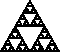
\includegraphics[scale=7]{sg.pdf}
\caption{An approximation of $\SG$}\label{fig:sg}
\end{figure}
The Sierpinski Gasket is a simple example of an iterated function fractal and can be described according to theorem \ref{thm:hutchinson} as the unique non-empty compact set $\SG\ssq\IR^2$ which is invariant under the three similitudes 
\[
  S_1(x,y)=\left(\frac{x}{2},\frac{y}{2}\right),\ 
  S_2(x,y)=\left(\frac{x+1}{2},\frac{y}{2}\right),\ 
  S_3(x,y)=\left(\frac{2x+1}{4},\frac{2y+\sqrt{3}}{4}\right),
\]
see figure \ref{fig:sg}. Since $\SG$ satisfies the (OSC), e.g. by taking the open equilateral triangle with corners $(0,0), (0,1)$ and $(1/2,\sqrt{3}/2)$, we obtain both 
\begin{equation}\label{eq:SGdimh}
  s=\dimh(\SG)=\frac{\ln 3}{\ln 2}
\end{equation}
and $\cH^s(\SG)\in(0,\infty)$ by a second appeal to Hutchinson's theorem. 

We will use the remainder of this section to establish the validity of the Einstein relation on $\SG$ with respect to the standard Laplace operator on $\SG$, which can be obtained in two different ways. In order to describe these constructions, we first need to fix some notation. 

Let $\scS=\{S_1,S_2,S_3\}$ as in section 1.1, set $\gS=\{1,2,3\}$ and denote by 
\[
  \gS^*:=\{\gep\}\cup\bigcup_{n\geq 1}\gS^n
\]
the free monoid consisting of all finite words over the alphabet $\gS$, where the monoid operation is given by concatenation and $\gep$ is supposed to represent the empty word. Using the monoid isomorphism 
$\gS^*\cong (\scS^*,\circ)$ given by extending 
$\gS\ni i\mapsto S_i\in\scS$, we can identify a word of length $l$,
\[
  w=w_1...w_l\in\gS^l,
\]
with the composition 
\[
  S_w:=S_{w_1}\circ...\circ S_{w_l}.
\]
By abuse of notation, we will therefore write $w(x)$ instead of $S_w(x)$. By an $n$-cell we understand the set $w(\SG)\ssq\SG$, where $w$ is a word of length $n$. Note that two different cells are either disjoint, or intersect in a single point which we will then call conjunction point, or one of them is completely contained in the other one. 

It is possible to approximate $\SG$ by a sequence of graphs $G_n$. Those graphs can be thought of as planar graphs with a triangle for each $n$-cell, where the vertices are the conjunction points between them. More precisely, let $G_n$ be the graph embedded in $\IR^2$ with vertex set $V_n$ inductively defined by
\begin{align*}
  V_0&:=
  \left\{(0,0),(0,1),\left(\frac{1}{2},\frac{\sqrt{3}}{2}\right)\right\}\\
  V_{n+1}&:=(S_1\cup S_2\cup S_3)(V_n),\ \ n\geq0.
\end{align*}
Additionally, set 
\[
  V*:=\bigcup_{n\geq0} V_n.
\]
Note that $V_0\ssq V_1\ssq...\ssq V_n\ssq ...$ and that
\[
  V_n=\bigcup_{w\in\gS^n} w(V_0).
\]
It also follows from the proof of Hutchinson's theorem that 
$d_H(V_n,\SG)\to 0$ as $n\to\infty$, so indeed, the graphs $G_n$ approximate $\SG$. 

\begin{figure}[h]
\centering
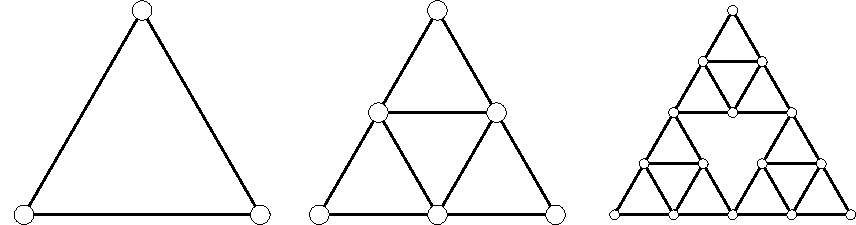
\includegraphics[scale=1]{gn.pdf}
\caption{The graphs $G_0,G_1,G_2$}\label{fig:gn}
\end{figure}

In $G_n$, connect two vertices $x,y\in V_n$ by a straight edge $xy$ iff they belong to the same $n$-cell, cf. figure \ref{fig:gn}, in which case we will call them neighbours and write $x\sim_n y$. By $E_n$ we mean the set of all edges in $G_n$. 



\subsection[Approximation by Dirichlet forms]{Approximation by Dirichlet forms\protect\footnote{The material in this section is an overview of the construction given in \cite[chapter I]{strichartz2006differential}}}

This analytic approach works by establishing so-called energy forms on graphs $G_n$ -- these are graph-theoretic discretisations of the Dirichlet form attached to the Laplace operator. For $n\in\IN$, define a bilinear form $\tilde\cE_n$ on $L^2(V_n)\cong \IR^{\# V_n}$ by 
\[
  \tilde\cE_n(f,g):=\sum_{xy\in E_n}(f(x)-f(y))(g(x)-g(y)), 
  \ \ \ f,g\in L^2(V_n).
\]
It is easy to check that this defines a local Dirichlet form on $L^2(V_n)$. As we will see, these bilinear forms are compatible with each other after a suitable renormalisation. Starting from $\tilde\cE_0$, consider a function 
$u\in\IR^3\cong L^2(V_0)$. Under all possible extensions 
$\tilde u$ to $\IR^6\cong L^2(V_1)$, which function is the harmonic extension of $u$, i.e. minimises $\tilde\cE_1[\tilde u]$? 

\begin{figure}[h]
\centering
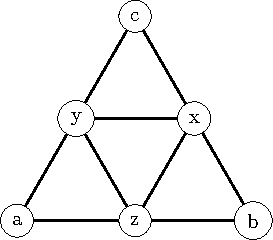
\includegraphics[scale=1]{g1.pdf}
\caption{The values of $u$ on $V_1$}\label{fig:g1}
\end{figure}

To answer this question, we label each vertex in $V_0$ by its value under $u$, say $a,b,c$ and each vertex in $V_1\setminus V_0$ by its value under $\tilde u$, say $x,y,z$ as in figure \ref{fig:g1}. Since we assume $u$ to be a fixed given function, the values $a,b,c$ are fixed, and we obtain 
\begin{multline}\label{eq:E1}
  \tilde\cE_1[\tilde u]=\left[(x-b)^2+(x-c)^2+(y-a)^2+(y-c)^2+(z-a)^2+(z-b)^2\right.\\
  \left.+(x-y)^2+(y-z)^2+(z-x)^2\right]
\end{multline}
Finding the minimising values for $x,y,z$ now becomes an exercise in multivariable calculus. Setting the partial derivatives equal to 0 yields the following system of linear equations:
\begin{align*}
  \begin{array}{c}
    8x=2(b+c+y+z)\\
    8y=2(a+c+x+z)\\
    8z=2(a+b+x+y)\\
  \end{array}\Longleftrightarrow
  \begin{array}{c}
    5x=a+2b+2c\\
    5y=2a+b+2c\\
    5z=2a+2b+c\\
  \end{array}
\end{align*}
Plugging this solution as $\tilde u$ in \eqref{eq:E1} to evaluate $\tilde\cE_1[\tilde u]$ gives
\begin{align*}
  \tilde\cE_1[\tilde u]
  &=\frac{1}{25}\left[(a-3b+2c)^2+(a+2b-3c)^2+(-3a+b+2c)^2
    +(2a+b-3c)^2\right.\\
  &\qquad\qquad \left.+(-3a+2b+c)^2+(2a-3b+c)^2
    +(b-a)^2+(c-b)^2+(a-c)^2\right]\\
  &=\frac{30}{25}\left[a^2+b^2+c^2-ab-ac-bc\right]\\
  &=\frac{3}{5}\tilde\cE_0[u]
\end{align*}
Using the fact that the vertices in $V_{n+1}\setminus V_n$ are in $G_n$ only adjacent to vertices in $V_n$ and that 
$\tilde\cE_{n+1}$ is local on $n$-cells it is possible to show by induction that each $u\in L^2(V_n)$ allows for a unique harmonic extension $\tilde u\in L^2(V_{n+1})$ and that 
\[
  \tilde\cE_{n+1}[\tilde u]=\frac{3}{5}\tilde\cE_n[u]
\]
for all $n\geq0$. This allows us to renormalise the bilinear form $\tilde\cE_n$ via 
\[
  \cE_{n+1}:=\left(\frac{3}{5}\right)^n\tilde\cE_n
\]
thus ensuring $\cE_{n+1}[\tilde u]=\cE_n[u]$ and therefore
$\cE_{n+1}[\hat u]\geq\cE_n[u]$ for any extension $\hat u$ of $u$.

Consider now any function $u:V^*\to\IR$ and denote its restriction to $V_n$ by $u_n$. Then, $\cE_n[u_n]$ is a nondecreasing sequence of nonnegative real numbers and therefore converges against 
\[
  \cE[u]:=\lim_{n\to\infty} \cE_n[u_n]\in[0,\infty].
\]
Define $\scD(\cE)$ to be the set of all functions $u:V^*\to\IR$ for which this limit is finite. It can be shown that $u\in\cE$ implies that $u$ is H\"older continuous and can therefore be uniquely extended to a continuous function on all of $\SG$. By abuse of notation we shall denote this extension by $u$ as well and set $\cE[u]:=\cE[u|_{V^*}]$ whenever the right-hand side is defined. Hence, by polarisation, we obtain a bilinear form $\cE(\cdot,\cdot)$ on $\scD(\cE)$. 

We further introduce the measure 
$\mu(\cdot):=\cH^s(\SG)^{-1}\cH^s(\cdot)$ on $\SG$. It is possible to show that the biliner form $(\cE,\scD(\cE))$ is a local regular Dirichlet form on $L^2(\SG,\mu)$ which in turn is attached to an operator as in equation \eqref{eq:DFtoOp}. This operator is what is known as standard Laplacian on $\SG$, and its spectral dimension is known to be $\frac{\log 3}{\log 5}$ (see e.g. \cite[section 3.5]{strichartz2006differential} or \cite{kigami1993weyl}). 

\subsection[Approximation by random walks]{Approximation by random walks\protect\footnote{The material in this section is an overview of the construction given in \cite[chapter II]{barlow1998diffusions}}}

It remains to discuss the walk dimension of the diffusion process generated by the standard Laplace operator on $\SG$. Once again, this construction uses the approximating graphs $G_n$. 

For $n\geq0$, let $Y^{(n)}_k, k\in\IN_0$ be a simple random walk on $G_n$, i.e. given $Y^{(n)}_k=v\in V_n$, the process has equal probability to jump to each of the neighbours of $v$ in $V_n$. 

Take $v\in V_{n-1}$. Then, $v$ is contained in either 1 or 2 $(n-1)$-cells with conjunction points 
$\{x_1,...,x_i\}\ssq V_n\setminus\{v\}$, $i\in\{2,4\}$ depending on whether or not $v\in V_0$. Assume $Y^{(n)}_0=v$, $n\geq1$. The only way for $Y^{(n)}$ to leave the $(n-1)$-cells containing $v$ is via the points $\{x_1,...,x_i\}$. However, due to the symmetry, the probabilities of hitting $x_j, j=1,...,i$ first are equal. If we set 
\begin{align*}
  T^{n,m}_0&=\inf\left\{t\in\IN_0:Y^{(n)}_t\in V_m\right\}\\
  T^{n,m}_{k+1} &=\inf\left\{t\in\IN_0, t>T^{n+1,m}_k:
     Y^{(n)}_t\in V_m\setminus \left\{Y^{(n)}_{T^{n,m}_k}\right\}\right\},\ \ k\geq0,
\end{align*}
for $n>m$, then $\left(Y^{(n)}_{T^{n,m}_k}\right)_{k\in\IN_0}$ is a standard random walk on $G_m$ and therefore equal to 
$\left(Y^{(m)}_k\right)_{k\in\IN_0}$ in distribution. Using self-similarity and standard arguments for finite Markov-chains, it can be shown that $\PTE{T^{n,m}_{k+1}-T^{n,m}_k}=5^{n-m}$ and that $Y^{(n)}$ overcomes a distance (in graph metric) of $2^{n-m}$. The renormalised processes $X^{(n)}_k:=Y^{(n)}_{5^nk}$, $k\in\IN_0$ furthermore converge almost surely and uniformly on compact intervals to a continuous limit process $(X_t)_{t\geq0}$ with values in $\SG$. Additionally, the infinitesimal generator of $X$ coincides with the $\SG$-Laplacian introduced above. 
By construction, this process possesses a self-similarity, in the sense that $(X_{5t})_{t\geq0}=(2X_t)_{t\geq0}$ in distribution for sufficiently small $t$, and it is not hard to show that $\dimw(\SG,X)=\frac{\log 5}{\log 2}$

Putting everything together, we obtain for the Sierpinski gasket:
\[
  \frac{\log 3}{\log 2}=\dimh(\SG)=\dims(\SG,\gD)\dimw(\SG,X)
  =\frac{\log 3}{\log 5}\frac{\log 5}{\log 2},
\]
so indeed, the Einstein relation holds on $\SG$.


\section{The real line as bounded metric space}


Bounded metric spaces form the most important class of spaces for which too naive of an adaption of \eqref{eq:defdimwrong} does not yield useful results. Indeed, consider the metric measure space 
$X=(\IR,d_{\arctan},\gl^1)$, where the metric is defined as $d_{\arctan}(x,y)=|\arctan(x)-\arctan(y)|$. Since 
\[
  \tan:\left(\left(-\frac{\pi}{2},\frac{\pi}{2}\right),|\cdot|\right)\to(\IR,d_{\arctan}) 
\]
provides an isometry, we have $\dimh(X)=1$. On this space, we consider the negative of the usual weak Laplace operator, $-\gD_{\gl^1}$, defined by mapping a function $u\in H_0^1(\IR,\gl^1)$ to the unique $g\in L^2(\IR,\gl^1)$ such that
\[
  \int_\IR g\gp\,\Di\gl^1=\int_\IR \partial_x u\partial_x \gp\,\Di\gl^1
\]
holds for all $\gp\in H_0^1(\IR,\gl^1)$. Notice how this does not differ from the negative weak Laplace operator on $(\IR,|\cdot|,\gl^1)$ since we did not change the measure and both metrics induce the same topology. Thus, we get from Weyl's classical result $\dims(X,-\gD_{\gl^1})=\frac{1}{2}$ and from the arguments developed in section 2.1 that the associated Markov process is $2(B_t)_{t\geq0}$. 

It is now easy to see that \eqref{eq:defdimwrong} does not provide a useful notion of a walk dimension: Since $B_{\arctan}(x,R)=\IR$ for every radius $R\geq\pi$, the expression diverges to $\infty$. Even the more careful approach 
\[
  \lim_{R\nearrow\frac{\pi}{2}}\frac{\log \PTEp{\tau(R)}{0}}{\log R}
\]
runs into similar problems: Using the formula $\PTE{\tau([a,b])}=-ab$ for the exit time of a standard Brownian motion from the intervall $[a,b]\ni 0$, we get
\[
  \log \PTEp{\tau(B_{\arctan}(0,R))}{0}=2\log \tan R =\infty.
\]
However, the local walk dimension from definition \ref{def:dimw} works out quite elgantly: Setting $y=\arctan x\in\left(-\frac{\pi}{2},\frac{\pi}{2}\right)$, we obtain for some $\xi_1\in (y,y+r),\xi_2\in(y-r,y)$
\begin{multline*}
  \frac{\log \PTEp{\tau\big(B_{\arctan}(0,R)\big)}{0}}{\log r}
  =\frac{\log\left(\tan(y+r)-\tan y\right)}{\log r}+\frac{\log\left(\tan y-\tan (y-r)\right)}{\log r}\\
  =\frac{\log\frac{r}{\cos^2 \xi_1}}{\log r}+\frac{\log\frac{r}{\cos^2 \xi_2}}{\log r}
  =2-\frac{\log \cos^2 \xi_1}{\log r}-\frac{\log\cos^2 \xi_2}{\log r}
\end{multline*}
by using the mean value theorem. Taking the limit for $r\searrow0$ on both sides implies $\xi_1,\xi_2\to y$ and thus $\dimw(E,2B_t,x)=2$. 









%Chapter III.
\chapter{The Einstein Relation on Metric Measure Spaces}

This chapter is devoted to the investigation of the Einstein relation in the setting of an abstract mm-space. First, we focus on the behaviour under morphisms between mm-spaces to derive invariance properties of the Einstein relation. 

\section{The Einstein Relation under Lipschitz-isomorphisms}

\subsection{Lipschitz and mm-isomorphisms}

We will use this section to introduce two different categories $\mathsf{MM}_L$ and $\mathsf{MM}_{\leq1}$ whose objects are mm-spaces, but with different morphisms: 
\begin{itemize}
  \item In $\mathsf{MM}_L$, the set $\mathsf{MM}_L(X,Y)$ of morphisms from an object $X=(X,d_X,\mu_X)$ to another object $Y=(Y,d_Y,\mu_Y)$ is the set of all Lipschitz-continuous functions 
  \[ 
    \gp:\supp\mu_X\to\supp\mu_Y
  \]
  satisfying $\gp_*\mu_X=\mu_Y$.
  \item In $\mathsf{MM}_{\leq1}$, the set $\mathsf{MM}_{\leq1}(X,Y)$ of morphisms from an object $X=(X,d_X,\mu_X)$ to another object $Y=(Y,d_Y,\mu_Y)$ is the subset of $\mathsf{MM}_L(X,Y)$ consisting of all contraction maps (i.e. Lipschitz-continuous functions $f$ with $\Lip_f\leq1$, cf. \eqref{eq:Lip}).
\end{itemize}
In both of those categories, composition of morphisms is to be understood as the usual composition of maps. By definition, $\mathsf{MM}_{\leq1}$ is a subcategory of $\mathsf{MM}_L$. Considering the usual notion of isomorphism, both categories give rise to a meaningful concept of isomorphy for mm-spaces: 
\begin{defin}
  A Lipschitz-isomorphism between mm-spaces $(X,d_X,\mu_X)$ and $(Y,d_Y,\mu_Y)$ is a map 
  $\gp:\supp\mu_X\to\supp\mu_Y$ with $\gp_*\mu_X=\mu_Y$ satisfying the bi-Lipschitz condition
  \[
    \frac{1}{C}d_X(x,y)\leq d_Y(\gp(x),\gp(y))\leq Cd_X(x,y)
  \]
  for all $x,y\in\supp\mu_X$ and a constant $C\in[1,\infty)$ not depending on $x,y$.
  
  Similarly, an mm-isomorphism is defined to be a Lipschitz-isomorphism with constant $C=1$. (This coincides with definition 2.8 in \cite{shioya2016metric})
\end{defin}
As it turns out, Lipschitz-isomorphisms are precisely the isomorphisms in $\mathsf{MM}_L$, whereas mm-isomorphisms are the ones in $\mathsf{MM}_{\leq1}$.

Indeed, consider a Lipschitz-isomorphism $\gp:X\supseteq\supp\mu_X\to\supp\mu_Y\ssq Y$. By definition, this is an injective morphism from $\mathsf{MM}_L(X,Y)$. We need to show that $\gp$ is surjective to ensure the existence of a two-sided inverse in $\mathsf{MM}_L(Y,X)$. To this end, suppose there exists $y\in\supp\mu_Y\setminus \gp(\supp\mu_X)=:Z$. Since $\supp\mu_X$ is closed, so is its image under the homeomorphism $\gp$, and hence $Z\ssq \supp\mu_Y$ is open. As every open subset of $\supp\mu_Y$ is required to have positive measure, we obtain the contradiction
\[
  0<\mu_Y(Z)=\gp_*\mu_X(Z)=\mu_X\left(\gp^{-1}\left(\supp\mu_Y\setminus \gp(\supp\mu_X)\right)\right)=0.
\]
Hence, $\gp$ is indeed a bijection. Conversely, if $\gp$ is an isomorphism from $\mathsf{MM}_L(X,Y)$ then we get the lower Lipschitz-bound from the Lipschitz-continuity of $\gp^{-1}\in\mathsf{MM}_L(Y,X)$, thus showing that $\gp$ is also a Lipschitz-isomorphism. Analogously, the corresponding statement for mm-isomorphisms can be derived.

We will write $(X,d_X,\mu_X)\simeq (Y,d_Y,\mu_Y)$ if $X$ and $Y$ are Lipschitz-isomorphic, and 
$(X,d_X,\mu_X)\cong (Y,d_Y,\mu_Y)$ if they are mm-isomorphic. Trivially, $X\cong Y$ implies $X\simeq Y$. 

In what follows, we will always assume $\supp\mu_X=X$.
\begin{rem}
  Of course, we always have $(X,d_X,\mu_X)\cong(\supp\mu_X,d_X,\mu_X)$ by virtue of 
  $\id:X\supseteq\supp\mu_X \to\supp\mu_X$. The restriction $\supp\mu_X=X$ becomes necessary for the Einstein relation since $\dimh(\supp\mu_X)$ might be strictly smaller than $\dimh(X)$, the term appearing in the Einstein relation \eqref{eq:ER}. We will later see (Proposition \ref{prop:mmiso}) that the Einstein relation is invariant under Lipschitz-isomorphisms which provides some motivation to circumvent this restriction by considering the relation
  \[
    \dimh(\supp\mu_X)=c\dims(\supp\mu_X,A)\dimw(\supp\mu_X,M)
  \]
  instead of \eqref{eq:ER}.
\end{rem}

\subsection{Transport of structure}

Given two mm-spaces $(X,d_X,\mu_X)$ and $(Y,d_Y,\mu_Y)$ with a map $\gp:X\to Y$, where a suitable operator 
$A:L^2(X,\mu_X)\supseteq\cD(A)\to L^2(X,\mu_X)$ satisfies the Einstein relation with constant $c$ on $X$. How can we transport $A$ alongside $\gp$ to become an operator on $L^2(Y,\mu_Y)$, and which restrictions do we need to impose on $\gp$ to ensure that this transport of structure is compatible with the theory from chapter 1?

Note first that any bimeasurable bijection $\gp:(X,d_X,\mu_X)\to(Y,d_Y,\mu_Y)$ induces by precomposition an operator
\begin{align*}
  \gp_*:L^2(Y,\nu)&\to L^2(X,\mu)\\
  f(y)&\mapsto(f\circ\gp)(x)
\end{align*}
which is an isometric isomorphism because $\gp^{-1}:Y\to X$ induces its inverse and because of
\begin{equation}\label{eq:isometry}
  \left\|\gp_*f\right\|_{L^2(X,\mu_X)}^2
  =\int_X |f(\gp(x))|^2\,\Di\mu_X
  =\int_Y |f|^2\,\Di\gp_*\mu_X
  =\int_Y |f|^2\,\Di\mu_Y
  =\|f\|_{L^2(Y,\mu_Y)}^2,
\end{equation}
by the change of variables formula for Lebesgue integrals. 

Denote by $\IL(H)$ the set of all partially defined linear maps (not necessarily bounded) on a Hilbert space $H$. Given an operator $A\in\IL(L^2(X,\mu_X))$, we can now contruct an operator $\gp_{\IL} A\in\IL(L^2(Y,\mu_Y))$ by conjugating with $\gp_*$. More explicitly, we define the map
\[
  \gp_{\IL}:\IL(L^2(X,\mu))\to\IL(L^2(Y,\mu))
\]
where $(\gp_{\IL} A)f:=(\gp_*^{-1}\circ A\circ\gp_*)f$ and $\cD(\gp_{\IL} A)=\gp_*^{-1}(\cD(A))$. Note that $\gp_L$ is again a bijection with inverse given by $\gp_L^{-1}=(\gp^{-1})_L$ and that this bijection restricts to the spaces of bounded linear operators. 

It follows immediately that $\cD(\gp_{\IL} A)$ is dense iff $\cD(A)$ is, and $\gp_{\IL} A$ is self-adjoint iff $A$ is. Indeed, consider arbitrary $f,g\in\cD(\gp_{\IL} A)$ with $f=\gp_*^{-1}(\bar f)$ and $g=\gp_*^{-1}(\bar g)$, where $\bar f, \bar g\in \cD(A)$. Then, applying \eqref{eq:isometry}, we have
\[
  \left<(\gp_{\IL} A)f,g\right>_{L^2(Y,\mu_Y)}
  =\left<\gp_*^{-1}A\gp_*\gp_*^{-1}\bar f,\gp_*^{-1}\bar g\right>_{L^2(Y,\mu_Y)}
  =\left<A\bar f,\bar g\right>_{L^2(X,\mu_X)}
\]
and we can perform the same calculations for $\left<f,(\gp_{\IL} A)g\right>_{L^2(Y,\mu_Y)}$, thus establishing the claimed equivalence. It is equally straightforward to check that the resolvent sets and the eigenvalues of $A$ and $\gp_{\IL} A$ coincide: Consider $\gl\in\rho(A)$, that is, 
$(\gl-A)^{-1}$ is a bounded linear operator on $L^2(X,\mu_X)$. To show $\gl\in\rho(\gp_L A)$, we consider
\[
  (\gl-\gp_L A)^{-1}
  =\left(\gl-\gp_*^{-1}A\gp_*\right)^{-1}
  =\left(\gp_*^{-1}(\gl-A)\gp_*\right)^{-1}
  =\gp_*^{-1}(\gl-A)^{-1}\gp_*
  =\gp_L(\gl-A)^{-1}
\]
which is a bounded linear operator on $L^2(Y,\mu_Y)$. If $\gl\in\IC$ happens to be an eigenvalue of $A$ with eigenfunction $f\in L^2(X,\mu_X)$, then -- as might have been expected -- $\gp_*^{-1}f$ is an eigenfunction of 
$\gp_L A$ to the eigenvalue $\gl$ as well. This can easily be checked by calculating
\[
  (\gp_L A)\big(\gp_*^{-1}f\big)=\gp_*^{-1}Af=\gl(\gp_*^{-1}f).
\]


Moreover, $\gp_{\IL}$ respects operator semigroups: If $(T_t)_{t\geq0}$ is a strongly continuous contraction semigroup on $L^2(X,\mu)$ with generator $(-A,\cD(A))$ then $(\gp_{\IL} T_t)_{t\geq0}$ is a semigroup with the same properties on $L^2(Y,\mu_Y)$ and with generator $(-\gp_{\IL} A,\cD(\gp_{\IL} A))$. Indeed, the semigroup property is trivial to check. For contractiveness, note that for $L^2(Y,\mu_Y)\ni f=\gp_*^{-1}\bar f$ with 
$\bar f\in L^2(X,\mu_X)$
\[
  \left\|(\gp_{\IL}T_t)f\right\|_{L^2(Y,\mu_Y)}
  =\left\|\gp_*^{-1}T_t\gp_*\gp_*^{-1}\bar f\right\|_{L^2(Y,\mu_Y)}
  =\left\|T_t\bar f\right\|_{L^2(X,\mu_X)}
  \leq\|\bar f\|_{L^2(X,\mu_X)}=\|f\|_{L^2(Y,\mu_Y)}.
\]
For strong continuity, we calculate
\[
  \left\|\gp_{\IL} T_t f-\gp_{\IL} T_0 f\right\|
  =\left\|\gp_*^{-1}(T_t\gp_*f-\gp_*f)\right\|
  =\left\|T_t(\gp_*f)-(\gp_*f)\right\| \to 0
\]
for $t\searrow 0$ and arbitrary $f\in L^2(X,\mu)$, and verifying the generator works analogously. 

Note however that a bi-measurable bijection $\gp$ does not respect enough structure to ensure that 
$\gp_\IL \sqrt{A}$ generates a regular Dirichlet form if and only if $\sqrt{A}$ does -- recall that this means the density of $\cD(\sqrt{A})\cap C_c(Y)$ in both $\cD(\sqrt{A})$ and $C_c(Y)$. To this end, suppose now that $\gp:X\to Y$ is a homeomorphism between $X$ and $Y$ (since both spaces are equipped with their Borel $\gs$-algebras, such $\gp$ is automatically bi-measurable and bijective). Similar to the case of $L^2$-spaces, this induces an isometric isomorphism $\gp_*:C_0(Y)\to C_0(X), \gp_*(f)=f\circ\gp$ between algebras of continuous functions vanishing at infinity, equipped with sup-norm $\|\cdot\|_{C_0}$. This isomorphism restricts to the subalgebras of compactly supported continuous functions $C_c(X)$ resp. $C_c(Y)$. 

\begin{lem}
  With the notation just introduced, if the Dirichlet form on $L^2(X,\mu_X)$ defined by 
  \[
    \cE(f,g):=\left<\sqrt{A}f,\sqrt{A}g\right>_{L^2(X,\mu_X)}\ \text{ for } f,g\in\cD(\sqrt{A})
  \]
 is regular then so is the Dirichlet form on $L^2(Y,\mu_Y)$ defined by 
 \[
   (\gp_\IL)^*\cE(\bar f,\bar g):=\left<(\gp_\IL\sqrt{A})\bar f,(\gp_\IL\sqrt{A})\bar g\right>_{L^2(Y,\mu_Y)}\ \text{ for } \bar f,\bar g\in\gp_*^{-1}(\cD(\sqrt{A})).
 \]
\end{lem}
\begin{proof}
  We need to show that the intersection of $\cD(\gp_\IL\sqrt{A})=\gp_*^{-1}(\cD(\sqrt{A}))$ and $C_c(Y)$ is dense both in $C_c(Y)$ w.r.t $\|\cdot\|_{C_0(Y)}$ and in $\cD(\gp_\IL\sqrt{A})$ w.r.t. $((\gp_\IL)^*\cE)_1$ as introduced in definition \ref{defin:DF}.
  
  For the first part, take $C_c(Y)\ni f=\gp_*^{-1} g$ for $g\in C_c(X)$. Then, there exists a sequence $(g_n)_{n\in\IN}\ssq \cD(\sqrt{A})\cap C_c(X)$ with $\|g_n-g\|_{C_0(X)}\to 0$ as $n\to\infty$. Since $\gp_*^{-1}$ is isometric, we conlude that $f_n:=\gp_*^{-1}g_n\in \cD(\gp_\IL\sqrt{A})\cap C_c(Y)$ converges to $f$ in 
  $\|\cdot\|_{C_0(Y)}$.
  
  For the second part, we analogously take $\cD(\gp_\IL\sqrt{A})\ni f=\gp_*^{-1} g$ for $g\in\cD(\sqrt{A})$. By regularity of $\cE$, there exists again a sequence $(g_n)_{n\in\IN}\ssq\cD(\sqrt{A})\cap C_c(X)$ with $\cE_1[g_n-g]\to 0$ as $n\to\infty$. Setting $f_n:=\gp_*^{-1} g_n\in\cD(\gp_\IL\sqrt{A})\cap C_c(Y)$, we obtain
  \begin{align*}
    ((\gp_\IL)^*\cE)_1[f_n-f]
    &=\left\|\left(\gp_\IL\sqrt{A}\right)(f_n-f)\right\|_{L^2(Y,\mu_Y)}^2
        +\|f_n-f\|_{L^2(Y,\mu_Y)}^2\\
    &=\left\|\gp_*^{-1}\sqrt{A}\gp_*\gp_*^{-1}(g_n-g)\right\|_{L^2(Y,\mu_Y)}^2
        +\|\gp_*^{-1}(g_n-g)\|_{L^2(Y,\mu_Y)}^2\\
    &=\left\|\sqrt{A}(g_n-g)\right\|_{L^2(X,\mu_X)}^2+\|g_n-g\|_{L^2(X,\mu_X)}^2\\
    &=\cE_1[g_n-g]\to 0
  \end{align*}
  which concludes the proof.
\end{proof}

Putting everything together, we observe that $A$ satisfies the assumptions in \ref{cond:A} iff $\gp_\IL A$ does whenever $\gp:X\to Y$ is a homeomorphism, and then $\dims(X,A)=\dims(Y,\gp_\IL A)$. The spectral dimension is therefore stable under a very large class of transformations. As it turns out, this will not be the case for Hausdorff and walk dimension. 

\begin{prop}\label{prop:mmiso}
  Let $(X,d_X,\mu)$ and $(Y,d_Y,\nu)$ be complete separable locally compact path-connected metric measure spaces with $\supp\mu=X$ and $\supp\nu=Y$ that are Lipschitz-isomorphic by virtue of the map $\gp:X\to Y$. Suppose the Einstein relation with constant $c$ holds on $X$ with respect to an operator $(A,\cD(A))$ satisfying assumptions \ref{cond:A}. Then, the Einstein relation also holds on $Y$ with the same constant $c$ and with respect to $\gp_{\IL} A$.
\end{prop}
\begin{proof}
  As the Hausdorff dimension is invariant under bi-Lipschitz maps we obtain $\dimh(X)=\dimh(Y)$, and as observed above, $\dims(X,A)=\dims(Y,\gp_{\IL} A)$. So, it remains to show $\dimw(X,M)=\dimw(X,M^{(\gp)})$ where $M$ is a Hunt process associated to $A$ and $M^{(\gp)}$ is one associated to $\gp_{\IL} A$. 
  
  We consider the process $N_t:=\gp(M_t)$. This process is a Hunt process with values in $Y$, and possesses the semigroup
  \[
    T_t^{(N)}f
    =\PTEp{f(N_t)}{\cdot}
    =\PTEp{(f\circ\gp)(M_t)}{\gp^{-1}(\cdot)}
    =T_t[\gp_*f](\gp^{-1}(\cdot))
    =\gp_*^{-1}T_t\gp_* f
    =(\gp_{\IL} T_t)f
  \]
  where we used the notation from the discussion above. 
  
  Thus, due to theorem \ref{thm:fukushima}, the processes $N$ and $M^{(\gp)}$ coincide up to their behaviour on a polar set. It is therefore enough to determine the walk dimension for $N_t$. By the bi-Lipschitz continuity of $\gp$, we obtain 
  \[
    \gp\left(B_X\left(x,C^{-1}r\right)\right)
    \ssq B_Y\big(\gp(x),r\big) 
    \ssq \gp\big(B_X(x,Cr)\big)
  \]
  where $C>0$ is the two-sided Lipschitz constant of $\gp$. Hence, $\tau_{C^{-1}r}^{(M)}\leq \tau_r^{(N)}\leq \tau_{Cr}^{(M)}$. From this, we get for all sufficiently small $r>0$
  \[
    \frac{\log Cr}{\log r}
     \cdot\frac{\log \PTEp{\tau_{Cr}^{(M)}}{x}}{\log Cr}
    \leq \frac{\log \PTEp{\tau_r^{(N)}}{\gp(x)}}{\log r}
    \leq \frac{\log C^{-1}r}{\log r}
     \cdot\frac{\log \PTEp{\tau_{C^{-1}r}^{(M)}}{x}}{\log C^{-1}r}.
  \]
  Taking the limit for $r\searrow0$ and applying a standard squeezing argument, we obtain $\dimw(X,M)=\dimw(Y,N)$. 
\end{proof}
\begin{rem}\label{rem:ToS}
  Note that we only needed the bi-Lipschitz property for determining 
  $\dimh$ and $\dimw$, whereas we only needed $\gp$ to be a homeomorphism in order to show that $M^{(\gp)}$ and $N$ share the same semigroup. This allows us in the following sections -- given a homeomorphism $\gp:(X,d_X,\mu_X)\to(Y,d_Y)$ -- to transport the complete structure needed for the Einstein relation by 
  \begin{itemize}
    \item Endowing $(Y,\mu_Y)$ with the push-forward measure $\gp_*\mu_X$.
    \item Mapping the generator $(A,\cD(A))$ to 
    $(\gp_LA,\gp_*^{-1}\cD(A))$, thus also mapping the generated semigroup $T_t$ to $\gp_LT_t$.
    \item Sending the Hunt process $M$ to $\gp(M)$. 
  \end{itemize}
  What we did so far ensures that all these constructions are compatible with each other. 
\end{rem}

From proposition \ref{prop:mmiso} we immediately obtain the following two corollaries:
\begin{cor}
  If $(X,d_X,\mu_X)\cong(Y,d_Y,\mu_Y)$ and the Einstein relation with constant $c$ holds on $X$ w.r.t. $(A,\cD(A))$ is an operator on $L^2(X,\mu)$, then it also holds on $Y$ with the same constant w.r.t. $\gp_{\IL}A$. 
\end{cor}
\begin{cor}
  If $X\ssq\IR^n$ and $d_1$ and $d_2$ are metrics which are induced by norms, then $\id_X:(X,d_1,\mu)\to(X,d_2,\mu)$ will preserve the constant in the Einstein relation.
\end{cor}
The second corollary follows from the well-known fact that all norms on a finite-dimensional Banach space are equivalent. 



\section{H\"older regularity and graphs of functions}

A natural question arising at this point is whether the invariance of the Einstein relation of propsition \ref{prop:mmiso} can be extended to a larger class of transformations. The following family of examples shows that this is not the case:

Consider a 1-dimensional continuous $\ga$-self-similar time-homogeneous strong Markov process $(M_t)_{t\geq0}$ over a suitable probability space $(\gO,\scA,\Prob)$. Here, $\ga$-self-similar for $0<\ga\leq1$ means that the processes 
$(M_t)_{t\geq0}$ and $\left(\xi^{-\ga}M_{\xi t}\right)_{t\geq0}$ have the same distribution. Denote by
\[
 \gr(M)=\gr(M_\cdot(\go)):=\left\{(t,M_t(\go)):t\geq0 \right\}\ssq \IR^2
\]
the graph of $M$ for fixed $\go\in\gO$. 

We endow $\gr(M)$ with the metric $d_\infty$ obtained by restricting the maximum norm $|(x,y)|_\infty=\max\{|x|,|y|\}$ of the surrounding space $\IR^2$ to $\gr(M)$. By construction, $\gr(M)$ comes with the natural map $\gp=\gp_\go:\IR_{\geq0}\to\gr(M)$ sending $t$ to 
$(t,M_t)$, providing a homeomorphism between $[0,1]$ and $\gr(M)$. 
While $\gp^{-1}$ is always Lipschitz-continuous since it is the projection onto the first coordinate, $\gp$ is in general only H\"older continuous with an exponent strictly smaller than 1. In fact, $\gp_\go$ is $\gc$-H\"older continuous if and only if the trajectory $M_\cdot(\go)$ is.

As pointed out in remark \ref{rem:ToS}, we can now transfer the analytic structure of section 2.1 on the half-line $\IR_{\geq0}$ via $\gp$ to 
$\gr(M)$. More explicitly, we have the measure $\gp_*\gl^1$ on $\gr(M)$ and an operator $\gp_L\gD_{\gl^1}$ acting on $L^2(\gr(M),\gp_*\gl^1)$ that generates the Hunt process $(\gp(W_s^t))_{s\geq0}$, where 
$(W_s^t)_{s\geq0}$ is a Wiener process independent from $M$ with start in $t\geq0$.

We note the following:
\begin{itemize}
  \item From \cite{liu1998hausdorff}, we get $\dimh(\gr(M))=2-\ga$ provided $M$ satisfies the technical conditions that there exist positive constants $K,K'$ and $0<r_0<1/3$ such that 
  \begin{equation}
    p(1,x,B(x,r_0))\geq K\ \ \text{ and }\ \ 
    p(1,x,B(x,r))\leq K'(1\wedge r)
  \end{equation}
  holds for all $x\in\IR$ and every sufficiently small $r>0$. Here, $p(t,x,A)$ denotes the transition function for $M$.
  \item As discussed in the last section we have
  \[
    \frac{1}{2}=\dims\left([0,1],-\frac{1}{2}\gD_{\gl^1}\right)
    =\dims\left(\gr(B),\Phi \left(-\frac{1}{2}\gD_{\gl^1}\right)\right),
  \]
  where we once again appealed to Weyl's classical results. 
  \item It remains to evaluate the walk dimension for $\gp(W_s)$ on 
  $\gr(M)$. As will be seen in the subsequent lemmata, we have 
  $\dimw(\gr(M_\cdot(\go)),\gp(W))=\frac{2}{\ga}$ $\Prob$-almost surely.
\end{itemize}
The Einstein relation -- despite holding with constant 1 on 
$\left([0,1],-\frac{1}{2}\gD_{\gl^1},W\right)$ -- therefore changes its constant under application of $\gp$ to
\[
  c(\ga)=\ga(2-\ga),\ \ \ga\in(0,1].
\]
\begin{lem}
  With the notation just introduced, we have 
  \begin{equation}\label{eq:BMdimw}
    \dimw\left(\gr(M_\cdot(\go)),\gp_\go(W),\big(T,M_T(\go)\big)\right)
    =\frac{2}{\ga}
  \end{equation}
  $\Prob$-almost surely for each $T>0$.
\end{lem}
\begin{proof}
  For brevity, set $x=x(\go)=(T,M_T(\go))\in\gr(M_\cdot(\go))$ and chose $r>0$ small enough for $B_\infty(x,r)\ssq\IR_{\geq0}\times\IR$, where 
  $B_\infty(x,r)$ stands for the open ball of radius $r$ around $x$ with respect to $d_\infty$.
  
  We begin by introducing the random times 
  $\gT^+_r\big(M_\cdot(\go),T\big),\gT^-_r\big(M_\cdot(\go),T\big)$ to denote the time where the Markov process $M$ first resp. last exits 
  $B_\infty(x,r)$ -- in other words,
  \begin{align}\label{eq:Theta}
    \gT^+_r\big(M_\cdot(\go),T\big)&:=\inf\left\{1\geq t>T:M_t\notin B_\infty(x,r)\right\}\notag\\
    \gT^-_r\big(M_\cdot(\go),T\big)&:=\sup\left\{0\leq t<T:M_t\notin B_\infty(x,r)\right\}.
  \end{align}
  Note first that by the Markov property of Brownian motion as well as by its time symmetry, these random variables are independent and the shifted random variables $\gT^+_r\big(B_\cdot(\go),T\big)-T,T-\gT^-_r\big(B_\cdot(\go),T\big)$ share the same distribution.
  
  By the standard result for the expectation of two-sided exit times for Brownian motion, we now obtain 
  \[
    \PTEp{\tau_{B_\infty(x,r)}^{(\gp(\bar B))}}{x}=-\big(T^+_r(\go)-T\big)\big(T^-_r(\go)-T\big)
  \]
  and consequentially
  \[
    \frac{\log  \PTEp{\tau_{B_\infty(x,r)}^{(\gp(\bar B))}}{x}}{\log r}
    =\frac{\log \big(\gT^+_r\big(B_\cdot(\go),T\big)-T\big)}{\log r}
     +\frac{\log \big(T-\gT^-_r\big(B_\cdot(\go),T\big))\big)}{\log r}.
  \]
  Therefore, it will suffice to show that $\Prob$-almost surely, 
  \begin{equation}\label{eq:limtwo}
    \lim_{r\searrow 0}\frac{\log \big(\gT^+_r\big(B_\cdot(\go),T\big)-T\big)}{\log r}
    =\lim_{r\searrow 0}\frac{\log \big(T-\gT^-_r\big(B_\cdot(\go),T\big)\big)}{\log r}=2,
  \end{equation}
  where it is enough to prove that one of the limits exist and equals 2. To this end, we consider more generally for a continuous function $f:[0,1]\to \IR$ the functionals
  \begin{align*}
    w:f(T)\mapsto &\liminf_{r\searrow0}\frac{\log\big(\gT^+_r(f,T)-T\big)}{\log r}\\
    W:f(T)\mapsto &\limsup_{r\searrow0}\frac{\log\big(\gT^+_r(f,T)-T\big)}{\log r}
  \end{align*}
  where $\gT^\pm_r(f,T)$ is defined analogously to \eqref{eq:Theta}. Suppose now that $f$ is $\ga$-H\"{o}lder 
  continuous ($0<\ga\leq 1$) in a given point $T\in[0,1]$, that is, there exists a constant $C>0$ and a 
  $\gep$-neighbourhood of $T$ such that for all $s$ inside this neighbourhood,
  \[
    |f(T)-f(s)|\leq C|T-s|^\ga
  \]
  is satisfied. This yields $\gT^+_r(f,T)\geq (r/C)^{1/\ga}$ for $r<\gep$ and therefore $(Wf)(T)\leq \frac{1}{\ga}$. Conversely, suppose that $f$ is not $\gb$-H\"{o}lder continuous ($\ga<\gb\leq 1$) in $T$. In particular, there exists a sequence $s_n=T+r_n\to T$ fulfilling the estimate 
  \[
    |f(T)-f(s_n)|>|T-s_n|^\gb=r_n^\gb,
  \]
  from which we deduce $\gT^+_{r_n}(f,T)\leq r_n^{1/\gb}$ and thus $(wf)(T)\geq\frac{1}{\gb}$. In particular, 
  $(Wf)(T)=(wf)(T)=\frac{1}{c}$ if $f$ is $\ga$-H\"{o}lder continuous in $T$ for all $\ga<c$ but not $\gb$-H\"{o}lder continuous for any $\gb>c$. 
  
  Having established this claim, the limit in equation \eqref{eq:limtwo} is a direct consequence of Paley-Zygmunds regularity theorem for paths of Brownian motion. Moreover, this also shows that the limit does not depend on $T\in(0,1)$. 
\end{proof}



% Bibliography

\nocite{*}   %CAUTION!!!

\printbibliography
\addcontentsline{toc}{chapter}{Bibliography}


\end{document} 


